\section{Introducción y propósito}
El objetivo de este documento es facilitar la tarea y ayudar en el primer acercamiento a futuros estudiantes que tengan que continuar este proyecto. \\

Debido a la magnitud del proyecto (versiones, participantes, correcciones), damos una pequeña introducción histórica:
\begin{enumerate}
\item El problema del tráfico aéreo es un clásico de la literatura, aunque sigue sin haberse encontrado una solución óptima.
\item En el curso 2011/2012, Diego Ruiz Aguado y Gonazalo Quevedo García abordan el problema su Trabajo de Fin de Carrera con Antonio Alonso Ayuso como tutor. Más adelante se explicará como se dividió el proyecto.
\item El 05/2014 Antonio Alonso retoma el proyecto por su cuenta con el objetivo de reestructurar el código para facilitar su lectura (antes estaba todo en una sola clase de 3000 lineas) y solucionar errores en la lectura de la BBDD.
\item En el 15/16 Carlos Vázquez toma el proyecto como Trabajo de Fin de Grado con el objetivo de crear un heurístico que mejore las soluciones. Los tutores serán Abraham Duarte y Antonio Alonso Ayuso.
\end{enumerate}

\section{Detalles del problema}
A continuación se expone un resumen del problema y la estructura que tiene. Para más detalles consultar las memorias de los TFC de Diego o Rodrigo.

El problema de optimización trata de XXXXXXXXXXXXXx

los elementos que hay en el problema son los siguientes:
\begin{itemize}
\item \textbf{Árbol de escenarios :} 
\item \textbf{Vuelos: }
\item \textbf{Sectores: }
\item \textbf{Aeropuertos: }
\item \textbf{Conjuntos de tiempo: }
\end{itemize}

\section{Secciones del proyecto}
El proyecto se dividió en dos partes:
\begin{itemize}
\item \textbf{Reestructuración de la BBDD: }se partía de una base de datos mal estructurada y no relacional. Se creó una nueva versión sin valores duplicados y relacional. Esta parte se llevó a cabo en JAVA
\item \textbf{Definición del modelo: }al tratarse de un problema de optimización, existen una función objetivo y restricciones. Esto se llevó a cabo mediante CPLEX, una librería para resolver problemas de optimización en JAVA y C.\\

Para más infomración sobre la estructura de la BBDD o del funcionamiento de CPLEX, así como la función objetivo y restricciones del problema pueden verse en las memorias de los TFC de Diego o Rodrigo.
\end{itemize}

\section{Modelo}
El primer paso es pasar la BBDD antigua a la nueva. No vamos a dar más detalles porque es poco probable que nadie vuelva a repasar esta parte. Una vez ejecutado el JAVA, tenemos ya la BBDD nueva. Algunas tablas importantes que contienes:
\begin{itemize}
\item \textbf{Sobre aeropuertos: }
\begin{enumerate}
\item \underline{Airports}: id del aeropuerto y el sector donde se encuentra
\item \underline{AirportCapacitiesDiscrete: }capacidad de salida y llegada de cada aeropuerto
\item \underline{AirportCapacitiesTree: }recoge las variaciones de las capacidades de los aeropuertos y de despegue/aterrizaje que están en la tabla AirportCapacitiesDiscrete.
\end{enumerate}
\item \textbf{Sobre sectores: }
\begin{enumerate}
\item \underline{Sectors: }id de los sectores
\item \underline{SectorCapacitiesDiscrete: }capacidad de cada sector
\item \underline{SectorCapacitiesTree: }recoge la variación de capacidad de los sectores de SectorCapacitiesDiscrete
\end{enumerate}
\item \textbf{Sobre vuelos: }
\begin{enumerate}
\item \underline{Flights: }identificador, matrícula, momento de despegue, tiempos de retraso máximos, costes por cancelar o retrasarse 
\item \underline{Trajectories: }contiene los distintos ``trozos'' de los que se compone una trayectoria. Por ejemplo para acceder a las 2 primeras rutas posibles del vuelo con id=1, bastaría con hacer 
\begin{verbatim}
SELECT * FROM SchemaName.trajectories
where Flight_Id=1 and (Route_Id=1 or Route_Id=2);
\end{verbatim} 
\begin{figure}[h]
\centering
  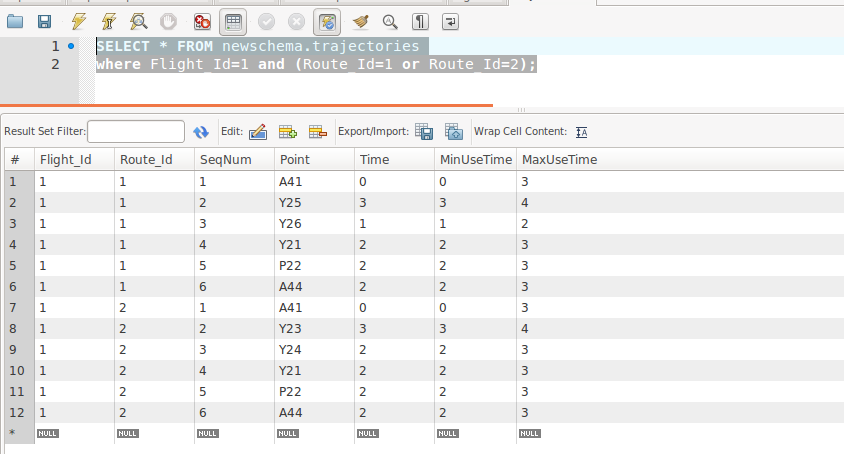
\includegraphics[width=1\textwidth]{./imagenes/trajectories}
  \caption{Trayectorias para un vuelo}
  \label{fig: Trayectorias para un vuelo}
\end{figure}
Aquí se pueden ver los segmentos de los que están compuestas las trayectorias para un vuelo determinado.
\item \underline{Waypoints: }a qué sector pertenece cada waypoint
\end{enumerate}
\item \textbf{Sobre árbol de escenarios: }\underline{ScenarioTree} tiene los nodos que forman el árbol de escenarios del modelo. Almacena los padres y el peso de cada nodo, además del tiempo en que se inician
\end{itemize}

\section{Detalles de implementación}
\subsection{Árbol de escenarios}
Como se dijo antes, hay un árbol de escenarios en el que para cada momento de tiempo puede haber varias configuraciones posibles. Como hay que moverse con frecuencia por el árbol para saber los padres y sucesores de un nodo, se descartó los árboles dinámicos. Se optó por una tabla hash de clave-valor que permiten acceder a un nodo determinado indicando solo la etapa de tiempo.
\subsection{Vuelos}
Son grafos dirigidos en el que los nodos representan a los waypoints y aeropuertos y las aristas son las uniones entre waypoints
\subsection{Conjuntos de tiempo}
Como se dijo antes, para cada arco y nodo hay que guardar 2 valores: el conjunto de tiempo y su intervalo (instantes de tiempo en los que puede llegar un vuelo y tiempo en recorrerlo). Los conjuntos de tiempo están implementados en un SortedSet. Para asociar cada conjunto a un vuelo se utiliza una tabla hash en la que el valor de búsqueda es el nodo/arco en cuestión. Los intervalos se almancenan directamente como 2 enteros (mínimo y máximo). Los conjuntos se van calculando en cada paso (ojo, no se pueden calcular los tiempos de un nodo sin haber calculado previamente los de los arcos incidentes)
